\documentclass[]{final_report}
\usepackage{graphicx}
\usepackage{float}
\usepackage{hyperref}
\usepackage[backend=biber, style=numeric]{biblatex}
\usepackage{url}
\usepackage{listings}
\usepackage{xcolor}

\definecolor{mygreen}{rgb}{0,0.6,0}
\definecolor{mygray}{rgb}{0.5,0.5,0.5}
\definecolor{mymauve}{rgb}{0.58,0,0.82}

\lstset{
	language=C++,
	basicstyle=\footnotesize\ttfamily,
	keywordstyle=\color{blue},
	commentstyle=\color{mygreen},
	stringstyle=\color{mymauve},
	numberstyle=\tiny\color{mygray},
	numbers=left,
	breaklines=true,
	tabsize=2,
	frame=single,
	captionpos=b
}

\lstdefinelanguage{GLSL}{
	sensitive=true,
	morekeywords=[1]{
		attribute, const, uniform, varying, break, continue, do,
		for, while, if, else, in, out, inout, float, int, uint,
		bool, true, false, lowp, mediump, highp, precision,
		void, discard, return, mat2, mat3, mat4, vec2, vec3,
		vec4, ivec2, ivec3, ivec4, bvec2, bvec3, bvec4, sampler2D,
		sampler3D, samplerCube, struct, gl_FragColor, gl_Position,
		gl_FragCoord
	},
	morekeywords=[2]{
		abs, acos, all, any, asin, atan, ceil, clamp, cos, cross,
		dFdx, dFdy, degrees, distance, dot, equal, exp, exp2,
		faceforward, floor, fract, greaterThan, greaterThanEqual,
		inversesqrt, length, lessThan, lessThanEqual, log, log2,
		matrixCompMult, max, min, mix, mod, normalize, not,
		notEqual, outerProduct, pow, radians, reflect, refract,
		sign, sin, smoothstep, sqrt, step, tan, texture2D,
		transpose, vec2, vec3, vec4
	},
	morecomment=[l]{//},
	morecomment=[s]{/*}{*/},
	morestring=[b]",
}

%%%%%%%%%%%%%%%%%%%%%%
%%% Input project details
\def\studentname{Henry Frodsham}
\def\reportyear{2025}
\def\projecttitle{A Concurrency Based Game Environment}
\def\supervisorname{Felix Bradley}
\def\degree{BSc (Hons) in Computer Science}
\def\fullOrHalfUnit{Full Unit} % indicate if you are doing the project as a Full Unit or Half Unit
\def\finalOrInterim{Final report} % indicate if this document is your Final Report or Interim Report

\begin{document}

\maketitle

%%%%%%%%%%%%%%%%%%%%%%
%%% Declaration

\chapter*{Declaration}

This report has been prepared on the basis of my own work. Where other published and unpublished source materials have been used, these have been acknowledged.

\vskip3em

Word Count (excluding code snippets): 6856

\vskip3em

Student Name:  Henry Frodsham

\vskip3em

Date of Submission: 19/12/25

\vskip3em

Signature: Henry.f

\newpage
\tableofcontents
\newpage
\chapter{Abstract}

This project is a Real Time Strategy (RTS) Game that focuses on using concurrency to provide a Local Multiplayer (LCM) experience through split screen. This project's primary aim is to provide steady performance regardless of the game state or number of players. a Secondary goal of this project is to provide an unlimited progression system for players such that players can progress through the game regardless of how long they have been playing. \newline

Users of this project will be able to play with 1-5 people on the same device and display, with 1 player on a keyboard and mouse and up to 4 on different controllers. This project assigns regions of the display to each player and automatically adjusts the aspect ratio and size of pre-existing regions when a player connects or disconnects. \newline

The primary motivation for this project Is the poor performance of pre-existing RTS games, even those that focus solely on a single player experience. Other RTS games experience input delay and stuttering issues as the game progresses due to high unit counts and complex interactions between units; for example, Stellaris by Paradox Interactive is well known by the RTS community to slow down significantly in the late game, to the point that the game cannot be played. \newline

Another Motivation for this project is the lack of split screen multiplayer in the RTS genre. split screen is often exclusively implemented in First Person Shooter (FPS) and racing Games although even those genres have seen a decline in split screen as of recently [2]. This project aims not only to revive the once believed feature of Split Screen but also to introduce it to the RTS genre, RTS is by nature a game with complex interactions between players and the addition of face-to-face communication could overall benefit the experience. \newline

By combining the technical innovations of modern game development with older styles of gameplay featuring more face to face interaction, this project demonstrates that performant, social RTS gaming is both viable and practical.


\subsection{ Aims and Objectives of the project}

 \textbf{Primary Objectives} \newline

\textbf{ Performance Optimization} \newline

 - achieve and maintain a consistent frame rate that initially matches that of the end users maximum refresh rate, and doesn't drop below the minimum video frame rate of 23FPS for any given scenario 

 - maintain low input latency that doesn’t spike above 50ms in any given scenario but should match that of the end users minimum input latency initially

 - produce no additional input delay or lag spikes regardless of the number of split screen instances running

 \textbf{local multiplayer functionality} \newline

 - implement a split screen local multiplayer system that allows for 1-5 players to play the game simultaneously

 - develop a robust input handling system that provides consistent input delay across all game instances

 \textbf{long term stability} \newline

 - optimize storage and management of in game units to minimize the performance degradation for a large numbers of units

 - prevent memory leaks to ensure the games memory usage doesn’t increase after extended play time, ultimately resulting in a program crash

 \textbf{user experience} \newline

 - design a clean UI that is free of clutter and provides a consistent experience across different input devices

 - implement a sensible text size and UI scaling to ensure visibility regardless of how small a given split screen instance is 

\textbf{Secondary Objectives} \newline

\textbf{Comprehensive real time strategy game}\newline

 - survey and respond to real time strategy players preferences
 
 - implement a progression system that allows players to continuously progress regardless of game stage
 
 \textbf{Comprehensive player interaction} \newline
 
 - allow players to form beneficial agreements 
 
 - implement an enmity system that expands on rivalries between players
 
 - allow transfers of resources between players
 

\subsection{Technology choices}

\textbf{Programming language: } C++ 20 \newline
\textbf{Chosen Compiler: } MSVC (with Visual Studio 2022) \newline
\textbf{Rendering Engine:} Ogre3D 1.14.2 (not to be confused with Ogre3D-next) \newline
\textbf{Input Handling Library:} SDL2 \newline
\textbf{UI and Overlay Library: } Ogre Overlay Component \newline
\textbf{Concurrency Library: } <Threading> library in C++ included in std libraries \newline
\textbf{Dependency installation and linking: } vcpkg library integrated with Visual Studio 2022 \newline

\chapter{Project Timeline}
\section{Term 1 Timeline}
\subsection{planned timeline}
\textbf{ Week 1:} write unit tests following TDD and setup build dependencies \newline
\textbf{Week 2:} research efficient ECS and event architecture \newline
\textbf{Week 3:} research input methods for controller and keyboard \newline
\textbf{Week 4:} code central event bus and ECS registry class \newline
\textbf{Week 5:} code input listeners + initial world and instance class \newline
\textbf{Week 6:} code initial split screen functionality and implement event queue \newline
\textbf{Weeks 7:} code entity factories and create entity components for ECS \newline
\textbf{Week 8-9:} create initial game map with partial game functionality \newline
\textbf{Weeks 10-11:} prepare interim transcript and improve implementation for presentation \newline
\subsection{Development timeline}
Week 1:

Research efficient event architecture (moved up from planned Week 2)

Week 2:

Implement event bus and event queue architecture (significantly ahead of schedule - originally planned for Weeks 4 and 6)

Weeks 3-5:

Input handling system implementation (timing not explicitly stated, but completed successfully)

Achieved reconnection for controllers
Automatic device recognition and configuration

Weeks 5-7:
Overlay system implementation

Attempted Dear ImGui integration with Ogre3D
Encountered compatibility issues with ApplicationContextBase
Researched and implemented alternative overlay solution (Ogre Overlay)
Weeks 7-9:
config system implementation

universal config system for storing and reading JSON files with nlohmann JSON

Week 10:
refinements to implementation

thread safety update to event architecture
refined input system with more debug information available

Week 11:

Create ECS registry class with demo implementation (delayed from planned Week 4)
Create ECS components with ECS factory (delayed from planned Week 7)

Week 12:

Initial split screen functionality implemented (delayed from planned Week 6)

Automatic viewport creation on device connection
Dynamic viewport resizing
Consistent aspect ratio maintenance



Not Completed in Term 1:

Partial game functionality (originally planned for Weeks 8-9)
Deferred to Term 2 to allow for REA pattern integration
 \subsection{Retrospective of Term 1s development}
 Over the development period in Term 1 there where some major differences between the planned timeline and actual development timeline. specifically, \newline
 - earlier development of event architecture fundamentals \newline
 - 2 week delay to implementing an overlay system \newline
 - delay to split screen functionality \newline
 - absence of partial game functionality \newline
 
 Term 1's development has brought to my attention that more careful analysis of planned technologies is required. Specifically, investigating implementations in other projects using similar technologies to me and which prerequisites are required or which existing technology could conflict. Another lesson learned from term 1's development is that more consistent contribution to reports and documentation is required in term 2's development, this way the CFD can easily be used to identify potential race conditions or design flaws.
 
 Despite these delays to the projects timeline, This project has reached a satisfactory end result for term 1. Large architectural groundwork has been completed, making way for development in term 2 along with recognizing REA as a new proven beneficial technology.
\section{Term 2 Timeline}
\textbf{Week 1: revisit term 1 implementation, refactor threading model and class communication} \newline
\textbf{Weeks 1-2: Research REA implementations, implement a basic scenario with multiple entities that can perform basic actions. } \newline
\textbf{Weeks 3-4: create a game world and a basic test scenario where each player is given starting units and starting territory} \newline
\textbf{Weeks 4-5: model and create simple REA actions for taking territory, attacking units, placing units.} \newline
\textbf{Weeks 6-7: create an undecorated UI, including context menus for actions that change depending on where the cursor is. settings and main menu screen} \newline
\textbf{Weeks 7-8: perform market analysis on experienced real time strategy players and implement suggestions as prototypes} \newline
\textbf{Weeks 8-9: perform user testing with prototypes to produce an unrefined game as the basis for the finished project} \newline
\textbf{Weeks 9-12: produce a shader complimenting a simplistic art style, implement a refined UI} \newline

\subsection{Development Timeline}
\textbf{Week 1: Refactored threading model using BSthreadPool, implemented per viewport overlays} \newline
\textbf{Week 2: Implemented a TDD scenario for REA, testing attacking scenarios. shell code for the transformation matrix and interaction evaluator} \newline
\textbf{Weeks 3-4: Designed the game globe, added visible cursors to controllers. refactored input translator to allow communication to the render thread} \newline
\textbf{Weeks 4-5: Refactored threading model, implemented per viewport overlays} \newline
\textbf{Weeks 6-7: Created the interaction wheel, created generic functionality for ui elements to be pressed or hovered over.} \newline
\textbf{Weeks 7-8: Performed market analysis via conversations with RTS players, implemented fixes to rendering errors, misaligned button text and a visual representation of selected units} \newline
\textbf{Weeks 8-9: Following Weeks 7-8, I reached out again and implemented unit movement functionality, cities. And blocked users from placing units in the ocean.} \newline
\textbf{Week 10: Implemented REA, added specialised entity components for cities and units. Added a specialised entity loop. } \newline
\textbf{Weeks 10-12: Created a fragment shader responsible for showing enemy units as different colours. Also implemented attacking units functionality. Cities now produce units passively instead of giving the player access to an infinite amount} \newline

\subsection{Retrospective of Term 2s development}
Term 2's development followed the planned timeline considerably more closely than Term 1, with the majority of features being implemented within their intended windows. However, a small number of development choices resulted in minor deviations from the original plan. Those being: \newline
- A delay to a working REA implementation \newline
- A delay to producing a playable prototype \newline
- A switch from a visual fidelity shader to a shader responsible for colouring enemy units \newline

The most notable of these was a delay to the REA implementation. Rather than introducing REA alongside the game world in Weeks 3–5 as planned, the decision was made to delay the technology until a functional UI had been created. This was a deliberate trade-off: without any observable visual representation of any entity interactions using REA, validating the correct desired behaviour of entity interactions would have been significantly harder, from both a user testing and development standpoint.

A consequence of this change to the development timeline was that a working prototype wasn't available at the start of the user testing phase. However, valuable feedback was still gathered following early user testing and I was able to respond to this feedback with fixes to the UI and a visual representation of selected units. More feedback was gathered in the following weeks 8-9, bringing about major changes to the final implementation with the addition of cities that passively generate units.


The final major change to the plan for term 2s development was the decision to implement a fragment shader focused on colouring enemy units instead of one focused on visual fidelity. This decision was made due to the development priorities of the project, those being prioritising function over visual fidelity. If I had opted for a fragment shader focused on fidelity then the overall performance of the project would suffer, since colouring enemy units could only otherwise be done with an inefficient CPU heavy loop, thus I opted to solve this problem efficiently with the fragment shader rather than compromise performance.



\newpage
\chapter{Technical Literature Survey}
\section{Core Real time Strategy Game Architecture}
\subsection{Entity Classification and Entity Interactions}
RTS games are heavily focused on "units" such as friendly soldiers or a farm that produces food for the player every set amount of time. Each "unit" within an RTS game is highly varied in its behaviour, but may share common attributes such as a position on the screen and a 3D model. \newline
A major challenge faced during the development of RTS games is storing and handling entities differently according to their behaviour; without an efficient method to store and compute the behaviour of large numbers of entities, it causes significant performance concerns as the number of entities increases. Despite there being pre-existing methods to tackle this problem, it is still common to see an "end year" or a "victory year" implemented within RTS games to prevent the number of units growing too large. The primary reason for RTS games still implementing a limit to game time is the inclusion of highly detailed 3D meshes where they would otherwise be unnecessary. \newline
One popular choice used for entity storage in the development of RTS games is ECS (Entity Component System), since it not only provides efficient storage but also offers the perfect solution for classifying modular entity behaviour through its component system. ECS's component system allows developers to modularise entities into specific behaviours that can easily be reused or removed from an entity to modify its behaviour. \newline
ECS is a powerful choice for real-time strategy games due to entity and component access being constant O(1) time, meaning that the time complexity of managing entities does not increase as more entities are added [5][6]. The reason for ECS achieving O(1) time is its employment of sparse sets --- a data structure consisting of two arrays, one sparsely filled with indices and another containing densely packed data. The indices in the sparse array point to entries in the dense array, and this bidirectional relationship is exploited by ECS to achieve O(1) time complexity for both retrieving an entity from a given component and retrieving a component from a given entity. Here is a visual representation of sparse set operation. \newline
\begin{figure}[H]
	\centering
	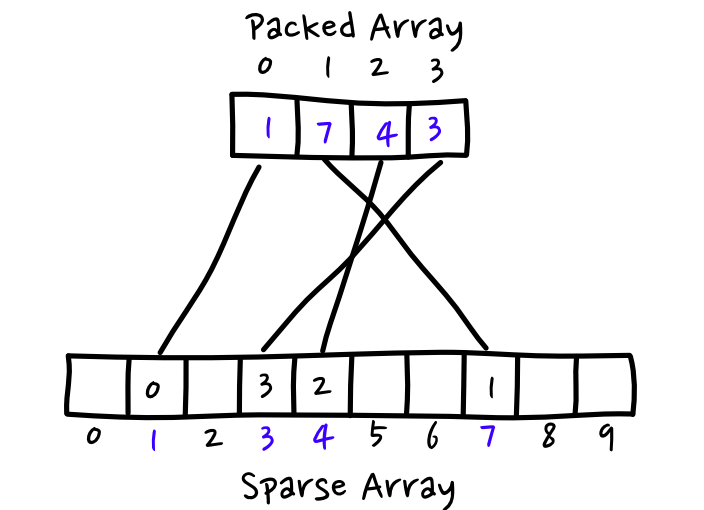
\includegraphics[width=0.7\linewidth]{screenshot001}
	\caption{sourced from Reference [1]}
	\label{fig:screenshot001}
\end{figure}
This diagram, however, does not fully illustrate how ECS implements sparse sets within its component system. Here is a diagram showing what a sparse set in a practical ECS implementation would actually look like. \newline
\begin{figure}[H]
	\centering
	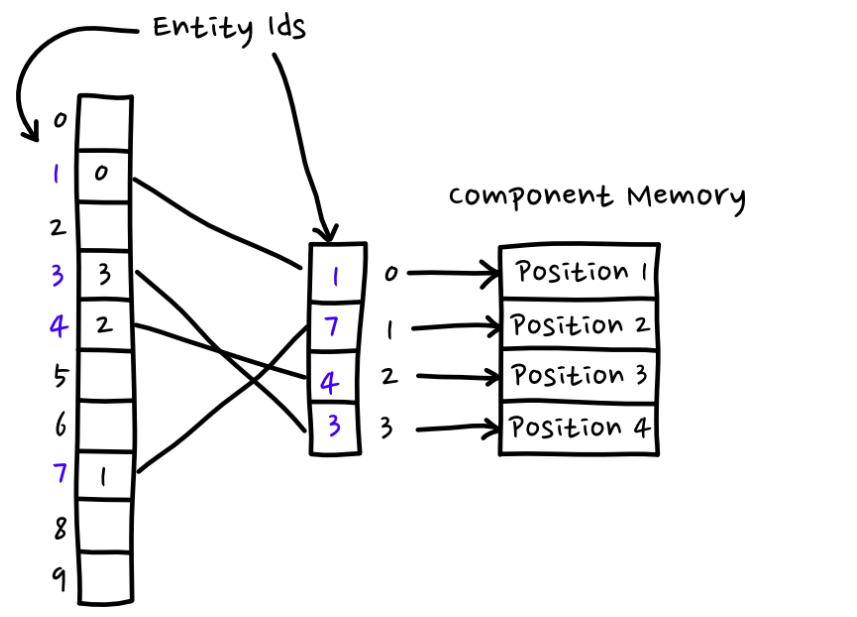
\includegraphics[width=0.7\linewidth]{screenshot002}
	\caption{sourced from Reference [1]}
	\label{fig:screenshot002}
\end{figure}
This diagram shows the relationship between the sparse set and a specific component, demonstrating O(1) lookup time. It is easy to assume that having two components would mean iterating over two different data structures; however, this is not the case --- instead, a new sparse set is created for each component [1]. \newline
However, evaluating actions between entities remains a significant challenge in RTS games. As the number of units increases, so too does the number of units implicated in any given action, thus exponentially increasing the processing time required. \newline
REA (Resource Entity Action) addresses this issue by modelling entity actions as resource exchanges, using transformation matrices to evaluate the resulting resources that affected entities hold after a given action. One example where REA proves useful is when two units in an RTS game attack each other --- a transformation matrix is used to calculate the resulting health of both entities. The REA pattern has been proven to provide a measurable performance advantage over implementations that do not employ it [2]. \newline
As mentioned previously, REA uses a matrix to evaluate actions as resource exchanges, but this is not always appropriate for every entity interaction. REA is primarily suited to routine calculations that are run most frequently and do not involve complex conditions or implications. For instance, an RTS game might use REA to calculate how much currency a factory unit should produce each second, since the conditions governing this are likely straightforward. \newline
 

\subsection{Split Screen Multiplayer Approaches }

Local cooperative multiplayer (LCM) involves multiple players sharing a single device, with each player receiving an independent portion of the screen controlled by their own input device. LCM is rare in the RTS genre and has seen a general decline across other genres such as FPS and racing, largely due to the expense and complexity of implementation. \newline
A significant technical challenge in LCM is managing multiple input devices simultaneously, as each device must be individually distinguishable and readable in parallel. Games requiring cursor or camera control typically rely on an input library to handle this, the most widely used being the GameInput library for Windows and Xbox [4]. SDL2 is a powerful choice for cross-platform compatibility, as it abstracts platform-specific code and keymaps automatically. \newline
Display splitting in LCM is typically handled through fixed-size screen segments, though unified views and distance-based splitting are alternative approaches used by some developers. \newline

\subsection{How I chose my implementations of ECS}
ECS can be implemented via various libraries in C++, two notable ones are Flecs and Entt. Entt uses sparse set to store entities whereas Flecs uses archetype.

Flecs has an advantage over Entt in terms of ease of use due to its query engine, making multiple entity and component retrievals easier to manage. Flecs is also included in the std library in c++ meaning it has the added advantage of not adding extra dependencies to my project.

However the main criteria im concerned with is their efficiency and space overhead. below is a table showing the space and time complexities of both libraries.

\textbf{Time Complexity} \newline
\begin{table}[!h]
	\centering
	\begin{tabular}{|l|c|c|}
		\hline
		\textbf{Operation} & \textbf{EnTT (Sparse Set)} & \textbf{Flecs (Archetype)} \\
		\hline
		\multicolumn{3}{|c|}{\textit{Entity Operations}} \\
		\hline
		Create Entity & $O(1)$ amortized & $O(1)$ \\
		\hline
		Delete Entity & $O(1)$ amortized & $O(1)$ \\
		\hline
		\multicolumn{3}{|c|}{\textit{Component Operations}} \\
		\hline
		Add Component & $O(1)$ amortized & $O(n)$\footnote{$n$ = entities in source archetype} \\
		\hline
		Remove Component & $O(1)$ amortized & $O(n)$\footnote{$n$ = entities in source archetype} \\
		\hline
		Get Component & $O(1)$ & $O(1)$ \\
		\hline
		Has Component (Check) & $O(1)$ & $O(1)$ \\
		\hline
		\multicolumn{3}{|c|}{\textit{Query/Iteration Operations}} \\
		\hline
		Iterate All Entities & $O(n)$ & $O(n)$ \\
		\hline
		View/Query Iteration & $O(n)$ & $O(n)$\footnote{With cached query} \\
		\hline
		Uncached Query Iteration & N/A & $O(A)$\footnote{$A$ = number of matching archetypes} \\
		\hline
		Create Cached Query & N/A & $O(E \log E)$ or $O(E)$\footnote{$E$ = total entities} \\
		\hline
		Create Uncached Query & N/A & $O(1)$ \\
		\hline
		Lookup Entity by Name & $O(1)$ & $O(1)$ \\
		\hline
		Component Registration & $O(1)$ & $O(1)$ \\
		\hline
	\end{tabular}
	\caption{Time Complexity Comparison - EnTT vs Flecs sourced using [5] and [6]}
\end{table}

\textbf{Space Complexity} \newline
\begin{table}[!h]
	\centering
	\begin{tabular}{|l|c|c|}
		\hline
		\textbf{Data Structure} & \textbf{EnTT (Sparse Set)} & \textbf{Flecs (Archetype)} \\
		\hline
		Entity Storage & $O(E)$\footnote{$E$ = max entity ID} & $O(E)$\footnote{$E$ = number of entities} \\
		\hline
		Component Storage & $O(E \cdot C)$\footnote{Sparse per component} & $O(E)$ (dense per archetype) \\
		\hline
		Sparse Index & $O(E)$ per component & N/A (uses archetype structure) \\
		\hline
		Archetype Storage & N/A & $O(A \cdot C)$\footnote{$A$ = archetypes, $C$ = avg components} \\
		\hline
		Query Cache & N/A & $O(Q \cdot A)$\footnote{$Q$ = queries} \\
		\hline
		Total Memory (avg case) & $O(E + E \cdot C_{avg})$ & $O(E + A \cdot C_{avg})$ \\
		\hline
		Total Memory (worst case) & $O(E \cdot C_{max})$ & $O(E \cdot C_{max})$ \\
		\hline
	\end{tabular}
	\caption{Space Complexity Comparison - EnTT vs Flecs sourced using [5] and [6]}
\end{table}



as can be seen on the table, Entt has the clear advantage in terms of speed and component overhead. whilst Flecs would be significantly easier to use and manage, my final choice for this project was Entt due to the performance focus of this project and any performance edge gained for such a critical architectural feature of this project must take priority.

\subsection{my use of ECS in this project}
ECS entities within this project are created using a factory pattern, where entities being created are split into their individual components then added in serial to the ECS registry to form the complete entity. below is a control flow diagram showing this process for the example cube.

\begin{figure}[H]
	\centering
	\includegraphics[width=0.7\linewidth]{"../Cube creation example"}
	\caption{a CFD of the example cube creation process}
	\label{fig:cube-creation-example}
\end{figure}

the example cube is made up of 2 ECS components. an OgreComponent and a MeshComponent, the OgreComponent contains an ogre scenenode (a universal object for any ogre entity) and the MeshComponent contains the mesh file path.
\subsection{how i chose my approach to split screen}
My chosen approach to split screen in this project is fixed size screen regions. Whilst a unified view of the game world would have been an acceptable choice for this project i decided against it to prevent confusion with multiple user interfaces appearing simultaneously on the same camera, the lack of individual camera control was also a factor considered since users wouldn't be able to focus in on specific game events. fixed screen sizes however do mean that a large display size is required to comfortably play with 4 or more players, careful design will be required for future development of this project to maximise accessibility for smaller displays.

\section{Concurrency in game Development}
\subsection{threading models}
threading models in game architecture is a fundamental architectural decision when designing games, threading models dictate how processing load is spread across different threads and thus spread across cpu cores. since modern CPU's almost always contain more than 1 core with most having 4-8, it's critical that these cores are utilized effectively to improve performance in game design. Single core dependence is a common issue faced in the RTS genre where only one cpu core is utilized due to architectural limitations, one example of this is Stellaris by Paradox Interactive which is known for poor late game performance since only 1 core is processing large numbers of game units.

one common approach to threading in game architecture is thread pooling, thread pools split tasks over a finite number of worker threads through a shared worker queue. one issue with thread pooling however is that two threads may access the same game resource at the same time since two threads could take a task accessing the same data. thread pooling is an extremely common approach in game design as if implemented correctly can ensure consistent core utilization across each cpu core.

another approach to threading models in games is the actor-entity model where each game object (actors) maintains their own internal state and reacts to messages. this approach avoids race conditions entirely as each thread processes actors without direct memory sharing meaning two threads will never access the same memory location. this approach does however introduce latency and ordering challenges since messages may arrive late or out of order.

\subsection{race condition avoidance}
Race conditions occur when two different threads attempt to enter the critical region at the same time e.g two threads access a variable at the same time. Race conditions are problematic since one thread could potentially read the value in the critical region whilst the other thread writes to the variable, causing thread 1’s read value of the variable to be incorrect.
Race conditions can be avoided in multiple different ways, the most notable being mutex locks where once a thread accesses a critical region it will lock access for other threads until it has exited. However, this creates problems of its own since one thread will be stuck waiting to enter the critical region and will sit idle until the other thread exits.

Another popular way game developers avoid race conditions is through Event architecture. Event architecture is composed of two main parts, Event Bus's and Event Queues with Event Bus's notifying subscribing functions immediately after an event is published then Event Queue's queuing up events to be processed in serial after its dispatch method is called. Event queues avoid race conditions by processing critical region accessing tasks one after the other thus preventing two accesses at the same time. 

\subsection{My approach}
My chosen Thread model for this project is thread pooling, each game instance will be assigned a thread that are synced at the end of each frame then reused for the next frame. Due to the nature of Ogre3d only being safely accessible from one thread i have seperated task queues into a local queue and a global queue. the local queue runs thread safe events only accessing that game instances data then the global queue is used to process non thread safe events such as moving a viewport.

whilst it can be said that Ogre3d only being able to be accessed from a single thread is a limitation of my project its important to note that down to a fundamental level GPU's run tasks in serial so issuing rendering commands in a multithreaded environment provides no significant advantage.
\section{Graphics/Rendering Engines}
\subsection{Comparison of commonly used Engines}
Game engines are systems that abstract complex rendering from developers. There are a variety of commercial and open source game engines available, each providing differing levels of abstraction. some well known choices being unreal engine and unity which are both considered heavyweight game engines since they abstract processes such as entity storage and concurrency. Open source and lightweight game engines are also widely used, the most popular being GoDot which abstracts considerably less than heavyweight game engines.

Whilst heavyweight game engines are the standard for large game development companies, they do introduce significant overhead and performance implications. The most notable example of this is with Unreal Engines 5's Nanite system for high detail meshes [3], some games use this system unnecessarily introducing no real visual fidelity benefit but causing significant performance degradation. One recent example of this is Borderlands 4, which has been criticized for poor performance on even high end hardware.

Lighter weight game engines are the clear choice when it comes to games focusing on performance. lighter weight game engines run with less overhead and systems such as entity storage are added via stand-alone libraries, following the "pay for what you use" principle. most game developers however still opt for heavyweight game engines despite a lack of real need for them, usually due to ease and thus cost of development. 

\subsection{Overlay and GUI Libraries}
Overlay systems are Rendering libraries that render 2d text or shapes over a 3d game world. Overlay systems are used by developers to show debug information such as current input device states and are also used to create GUI's for use by an end user. 

One popular Overlay system used in Game development is Dear Imgui. Dear Imgui is widely used to create debug overlays since it abstracts creating text inputs or drop down menus from developers, 
allowing sophisticated debug overlays to be created easily and conveniently by developers. Dear imgui is however unsuitable for creating a modern GUI for end user's since it's appearance is designed strictly to create tools, in addition to this Dear Imgui redraws the entire ui every frame which is unnecessary for menu buttons that largely remain static.

below is a picture of Dear Imguis UI
\begin{figure}[H]
	\centering
	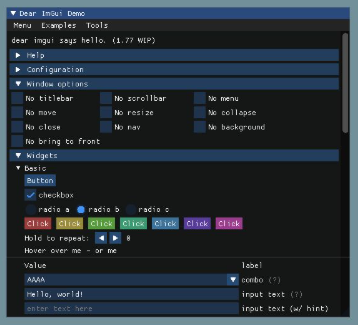
\includegraphics[width=0.7\linewidth]{screenshot003}
	\caption{}
	\label{fig:screenshot003}
\end{figure}

Another popular option is CEGUI, which is primarily used for GUI's.

\subsection{My Approach}
My chosen Overlay system is the Ogre Overlay library, which is natively included in Ogre3d. due to Ogre Overlay being part of Ogre3d's ecosystem it allows for convenient integration into this project, this has several benefits such as being able to create unique overlays for each viewport and inclusion within Ogre3d's rendering pipeline. Ogre Overlay is simplistic in terms of features such that Buttons and drop down menus must be created manually, although this means that a GUI library can be produced that is more specialised for this project's needs.

I had initially planned to use Dear Imgui to produce a debug overlay for this project, however due to unforeseen issues with integrating Dear Imgui with ogre i now use Ogre Overlay exclusively.
\section {Fragment shaders}
\subsection {comparison of commonly used fragment shader technologies}
Fragment shaders are a commonly used method for game developers to interact with the graphics pipeline without writing low level ARB assembly programs [14]. Fragment shaders execute for every pixel on screen and are responsible for per-pixel lighting, texture sampling and visual effects, running millions of times per frame [15]. A key feature of fragment shaders is that they execute solely on the GPU, allowing developers to leverage the massively parallel architecture of modern graphics hardware. This means otherwise CPU-heavy visual tasks can be delegated directly to the GPU, resulting in significantly lower CPU utilisation and a more efficient rendering pipeline overall.

Fragment shaders are written using shading languages, the most common being GLSL, HLSL and MSL. All three are written in a C style syntax, meaning developers familiar with one can switch between them with relative ease, as the differences are largely limited to keywords and platform-specific design philosophies rather than fundamentally different programming models [16]. Despite having similar syntax, the choice of shading language is typically dictated by the target platform rather than developer preference. GLSL is the standard for OpenGL and WebGL applications and is well suited for cross-platform development, HLSL is the primary language for DirectX and Xbox targets and is the default in Unity's built-in render pipeline, while MSL is exclusive to Apple hardware running Metal [17]. Beyond text-based shading languages, visual tools such as Unity Shader Graph and Unreal's Material Editor also exist as abstractions to these languages, trading low level control for faster development.

The differences between these approaches become particularly relevant when evaluating which is most appropriate for a given use case, as each carries distinct benefits and drawbacks in terms of platform support, performance control, and flexibility.

\begin{table}[h]
	\centering
	\renewcommand{\arraystretch}{1.4}
	\begin{tabular}{|p{2.5cm}|p{2.5cm}|p{2cm}|p{3.5cm}|p{3.5cm}|}
		\hline
		\textbf{Technology} & \textbf{Platform} & \textbf{Syntax Basis} & \textbf{Best For} & \textbf{Key Drawback} \\
		\hline
		GLSL & OpenGL, WebGL, Mobile & C & Cross-platform development & Often compiled differently across platforms causing inconsistent behaviour \\
		\hline
		HLSL & DirectX, Xbox, Unity & C & Windows and Xbox targets, Unity built-in render pipeline & Lack of cross-platform \\
		\hline
		MSL (Metal) & iOS, macOS, Apple Silicon & C++14 & Performance focused for  & Apple exclusive \\
		\hline
		WGSL & WebGPU & Rust-like & Modern web graphics & Newly introduced with limited functionality \\
		\hline
		Shader Graph (Unity) & Unity Engine & Node-based (Visual) & Rapid development & Limited low level control \\
		\hline
	\end{tabular}
	\caption{Comparison of common fragment shader technologies}
	\label{tab:shader_comparison}
\end{table}

As can be seen from the above table, GLSL is the only fragment shader language with native cross-platform support, and is purpose built for OpenGL. HLSL, while arguably the more widely used language in commercial game development, is restricted to the DirectX render system and therefore only supports Windows and Xbox, making it unsuitable for a project with cross platform capability. Similarly, MSL is exclusive to Apple's ecosystem and WGSL uses a non C like syntax. Due to this, the natural choice for a shader language within this project was GLSL, with the added benefit of being natively supported within Ogre3D, my chosen render engine. Ogre3D supports GLSL with its OpenGL render system, allowing fragment programs to be declared and referenced directly within material scripts, meaning parameters such as a player id can be referenced and modified from within the applications code. Furthermore, GLSL's C style syntax offers ease of development for a project written in C++ due to it removing the need to switch to a more rust like syntax with WGSL.

\subsection {Common uses for fragment shaders}

Fragment shaders are play a huge role in modern graphics pipelines, operating at the per pixel level to determine the final colour and appearance of rendered geometry. Fragment shaders where a huge improvement from early fixed-function pipelines which are described as inflexible and lacking the same configurability as fragment shaders [18]. Since then, fragment shaders have allowed developers to explore more complex lighting techniques and post processing effects with fragment shaders being described as the primary way of reaching visual fidelity in real time applications [15][16].

Fragment shaders play a central role in non photorealistic rendering, such as a game using a cartoon art style. A fragment shader could be used to automatically highlight edges of geometry with darkened lines by comparing neighbouring pixels for edge detection. This approach offers a flexible solution to a cartoon art style as fine details such as darkened lines are abstracted from the 3d modelling process, offering ease of development with no compromise to the rendering quality. 


One well known and advanced use of a fragment shader is ray marching with a Signed Distance Function (SDF). Where a scene is constructed entirely by mathematical functions instead of a traditional approach where geometry is made up of a list of triangles. An SDF is essentially an advanced implementation of a ray tracing function, returning a signed value of the distance to the closest geometry at a given 3d coordinate, the sign of the value indicates whether the 3d coordinate is inside or outside the geometry [19]. The Ray marching algorithm uses these properties to advance along the ray much like a typical ray tracing algorithm, however the SDF is called at each step to calculate a distance for the ray to skip, without any risk of skipping through any geometry. This process continues until the distance returned by the SDF is under the hit threshold, indicating a hit on a geometries surface.

This technique is used in real time procedural rendering, a technique where geometry is generated instead of loaded from a pre made mesh. In real time procedural rendering, defining geometry as a series of triangle meshes is impractical thus makes a perfect use case for the ray marching algorithm. A key advantage of this approach over traditional rasterisation is that all scene information is inherently accessible during shading via the SDF, whereas in a traditional rasteriser the polygons are processed in isolation with no awareness of other geometry. This limitation of standard rasterisation means that visual effects such as soft shadows must be precomputed and stored in a shadow map [20].With SDF's, the distance function can be called at any time thus making soft shadows and offer visual effects far more straightforward to compute. This technique can allow the entire rendering pipeline to run through fragment shaders, with no vertex data involved.

Below is an example implementation of the ray marching algorithm in GLSL.
\begin{lstlisting}[
	language=GLSL,
	caption={A GLSL example of Ray marching in a fragment shader)},
	label=lst:ray_marching
	]
	float rayMarch(vec3 ro, vec3 rd) {
		float depth = MIN_DIST;
		for (int i = 0; i < MAX_STEPS; i++) {
			float dist = sceneSDF(ro + depth * rd); 
			if (dist < EPSILON) return depth;       
			depth += dist;                          
			if (depth >= MAX_DIST) break;
		}
		return MAX_DIST; 
	}
\end{lstlisting}

The function takes a ray origin \texttt{ro} and a ray direction \texttt{rd} as inputs. 
Starting at \texttt{MIN\_DIST}, it iteratively advances a depth value along the ray by 
querying \texttt{sceneSDF} at the current position. If the returned distance falls below 
\texttt{EPSILON}, the ray is considered to have hit a surface and the current 
depth is returned. If the depth reaches \texttt{MAX\_DIST} without a hit, the maximum 
distance is returned to indicate a miss. The step size is not fixed, it equals the SDF 
value at each step.This is what makes sphere tracing efficient: the ray takes large 
steps through empty space and automatically slows down as it approaches a surface 
[19].

\subsection{My approach}

GLSL was chosen as the fragment shader language for this project for several reasons. As shown in \texttt{table 3.3}, it is the only shader language with native cross-platform support, which was a core requirement for this project. HLSL was ruled out due to its exclusivity to DirectX and therefore Windows and Xbox only. MSL is similarly restricted to Apple's ecosystem, and WGSL uses a Rust-like syntax rather than C-style, which would feel out of place in a C++ codebase. GLSL's C-style syntax keeps things consistent and reduces context switching during development. It also integrates directly with Ogre3D's OpenGL render system, allowing fragment programs to be declared within material scripts and have parameters like player ID passed in and modified from the application's code.

A simple implementation to display enemy units in different colours was chosen as the fragment shader for this project. Although the ray marching algorithm would have enhanced the visual fidelity, its implementation time would have been unacceptable given the project's focus on concurrency. As a result, a more practical fragment shader was used, prioritising function over visual fidelity.
That said, if I where to continue development of this project and eventually publish it then ray marching would be an excellent option to increase this projects visual fidelity.



\chapter{implementation}
\section{User interface}
A User Interface is a means for players to interact with a program. The user interface for this project reflects the rudimentary focus of the game implementation, with UI elements consisting of basic shapes with overlaid text.

The primary way players interact with the game is through the interaction wheel, a four-button radial menu revealed by pressing R on a keyboard or X on a controller. The interaction wheel was a suitable choice for this project given that the project supports both controllers and traditional keyboard and mouse. Since controllers offer comparatively less precision when moving the in-game cursor, I opted for a design that keeps all interaction options grouped as closely together as possible, reducing the distance the cursor needs to travel regardless of input method.

\subsection{User interface visibility across viewports}
The user interface was built using OGRE3D's overlay system, a 2D rendering layer included within OGRE's ecosystem that sits on top of the 3D viewport. Since overlays are tightly coupled to OGRE3D's rendering pipeline, all creation and management of overlay elements is handled exclusively on the render thread. Despite this constraint, a clear separation between UI elements is maintained by mapping them into distinct \texttt{Ogre::Overlay} instances based on the viewport they belong to. This is done using an \texttt{std::unordered map} with the \texttt{Ogre::Overlay} as the key and the \texttt{Ogre::Viewport} as the value, allowing for O(1) retrievals of Owned viewports.

This separation of overlay elements allows for an override of OGRE3D's \texttt{PreViewportUpdate}, a listener method called just before a viewport is rendered. Within this override, the overlay corresponding to the active viewport is made visible while all others are hidden, ensuring each overlay is only ever rendered to its intended viewport. This approach avoids the need for an extensive ownership check on the \texttt{Ogre::Overlay} and keeps the UI logic self-contained within the render thread. 

\begin{lstlisting}[
	language=C++,
	caption={iterating over stored the unordered map of viewports and overlays to show or hide accordingly (\texttt{Product.sln}, 
		\texttt{ViewPortUpdateListener.cpp})},
	label=lst:overlay visibility
	]
  // disable all the overlays, then enable the one that should be rendered
for (auto Viewport : InstanceViewports) {
	if (Viewport.second->Equals(evt.source)) {
		Viewport.first->show();
		char IdChar = Viewport.first->getName().back();
		PlayerId = IdChar - '0';
	} else {
		Viewport.first->hide();
	}
}
\end{lstlisting}
The \texttt{PreViewportUpdate} override receives a \texttt{RenderTargetViewportEvent} containing a reference to the active viewport, which is used to identify which overlay should be shown.The correct viewport is then identified by iterating over the \texttt{std::unordered map} where each one is checked against the active viewport from \texttt{RenderTargetViewportEvent}. Once the correct overlay is determined, \texttt{setVisible(true)} is called on it while the remaining overlays are hidden by calling \texttt{setVisible(false)}, ensuring no overlay is shown on an unintended viewport.

\subsection {User interface interaction}
With the overlay visibility system in place, the next challenge was implementing interactive UI elements within those overlays. OGRE3D's overlay system provides the basis for this through \texttt{Ogre::OverlayElement} and its subclasses, which represent individual UI components such as panels and text areas. However, OGRE3D's overlay system provides no built-in functionality for interactivity such as click detection or hover states, meaning any interactive behaviour had to be implemented manually.

The first challenge with implementing interactive UI elements was that \texttt{OverlayController} runs on the render thread, whilst cursor positions from input devices are evaluated inside the instance threads. The solution to this was to propagate cursor positions from the instance threads to \texttt{OverlayController} via a \texttt{MouseMovedEvent}, which carries both the identifier of the input device that moved and the viewport it belongs to. Using this information, \texttt{OverlayController} is able to narrow the cursor check down to the specific \texttt{Ogre::Overlay} associated with that viewport, rather than checking every overlay on every cursor movement. The relevant overlay is then retrieved by name, after which each contained \texttt{Ogre::OverlayElement} is iterated over and \texttt{findElementAt} is called to determine whether the cursor is positioned over it.

\begin{lstlisting}[
	language=C++,
	caption={performing a cursor check on elements contained within an Overlay (\texttt{Product.sln}, 
		\texttt{OverlayController.cpp})},
	label=lst:overlay cursor check
	]
void OverlayController::OverlayCursorCheck(CursorMovementEvent Event) {
	RenderSystem& RS = RenderSystem::GetInstance();
	ViewPortController* EventVPC = RS.FindViewPortFromDevice(Event.Device);
	
	// find the overlay specific to the device being moved (as to not check
	// everything for each device)
	std::string OverlayName = "UI_Overlay_" + std::to_string(Event.ThreadNumber);
	Ogre::Overlay* SpecificOverlay = OverlayMngr->getByName(OverlayName);
	
	Ogre::Overlay::OverlayContainerList ContainedElements =
	SpecificOverlay->get2DElements();
	
	for (Ogre::OverlayElement* Element : ContainedElements) {
		OverlayInfo* Info = nullptr;
		try {
			Info = OverlayInfos.at(Element->getName());
		} catch (std::exception e) {
			OverlayErrorReporter.EnqueueError(ErrorDetail::CreateError(ErrorCode::OVERLAY_MISSING_INFO));
			return;
		}
		
		if (Element->findElementAt(Event.RelativeXY[0], Event.RelativeXY[1])) {
			Info->Hovered = true;
			//pressing the overlay should always override hovering
			if (!Info->Pressed) {
				OverlayHovered(Element, Info);
			}
		} else {
			Info->Hovered = false;
			OverlayReleased(Element,Info);
		}
	}
}
\end{lstlisting}


The next challenge was implementing UI elements that had an effect when pressed. My initial approach to this problem was to store a pointer to the buttons state, either true or false indicating whether the button was pressed. A large issue with this approach was the lack of thread safety, \texttt{OverlayController} may write true to the value on one tick then false on another causing the instance thread to completely miss the trigger window where the value is true. The final chosen approach to this problem was a callback system, once the button had been pressed \texttt{OverlayController} calls a stored lambda callback to trigger the desired effect. For example, the main menu "play" button is registered with a lambda to queue a state change event, thus once the same tick that the button is pressed the application changes state with no chance of the instance thread not recognising it.

\section{concurrency}
This project has implemented Concurrent execution of each game instance, each game instance thread is managed using the thread pooling pattern. 

due to the current project state, each game instance thread is currently taking on a very small amount of processing responsibility. however, the system infrastructure required to distribute complex processing across game instance threads is implemented and once the project reaches a more complete state then the advantages of multi threading becomes more apparent.

\subsection{My race condition avoidance approach}
A race condition occurs when two threads running concurrently attempt to access 
the same shared resource at the same time, with at least one thread writing to 
that resource. Race conditions produce unexpected behaviour in multi-threaded 
programs, so prevention was a priority throughout the development of this project.

This project negates race conditions using event architecture, supported by the 
addition of event queues. All shared resource access is controlled via events, 
which act either as a request to complete a task or as an asynchronous 
information request. A typical example of this can be seen in 
Listing~\ref{lst:raytrace}, which demonstrates how events are used to prevent 
a race condition when issuing a ray trace command.

\begin{lstlisting}[
	language=C++,
	caption={Issuing a \texttt{StartRayTraceEvent} to the Render Queue to avoid 
		direct cross-thread access to Ogre3D (\texttt{Product.sln}, 
		\texttt{PlayerGeneralControl.cpp})},
	label=lst:raytrace
	]
	void PlayerGeneralControl::OnPress(PressActionCommand Cmd) {
		RenderSystem& RS = RenderSystem::GetInstance();
		std::vector<float> Position =
		std::vector<float>{Cmd.Context.MouseX, Cmd.Context.MouseY};
		RS.RenderQueue->Enqueue(StartRayTraceEvent(
		Position, PlayerTranslator->ManagedDevice,
		[](EventQueue* queue, EndRayTraceResultEvent Event) {
			queue->Enqueue(Event);
		},
		TriggerQueue));
	}
\end{lstlisting}

This code runs inside an instance thread and handles issuing a ray trace command 
to Ogre3D. If this code were to access Ogre3D directly, a race condition could 
occur if a separate thread accessed Ogre3D at the same time. Instead, a 
\texttt{StartRayTraceEvent} is issued to the Render Queue (the centralised queue 
for all Ogre3D interactions) and processed in serial with other Ogre3D 
interactions, preventing any direct cross-thread access.

A further element of race condition avoidance introduced in the second term of 
development is the use of a lambda callback for information requests. Since 
events are not processed immediately after being queued, it became necessary to 
find a solution to the absence of immediate information retrieval. As shown in 
Listing~\ref{lst:raytrace}, a lambda is created to queue an 
\texttt{EndRayTraceResultEvent} back to the sender, ensuring that 
\texttt{PlayerGeneralControl} is notified of the ray trace result in a thread 
safe manner.

This Approach to Race condition avoidance allows this project to remain lock free for the most part, making this project easily extendable. The only method directly accessed across threads is the Enqueue method in the event queue class, for this reason its necessary to use a mutex as seen below.

\begin{lstlisting}[
	language=C++,
	caption={Issuing a \texttt{StartRayTraceEvent} to the Render Queue to avoid 
		direct cross-thread access to Ogre3D (\texttt{Product.sln}, 
		\texttt{PlayerGeneralControl.cpp})},
	label=lst:raytrace
	]
  template <typename EventType>
void Enqueue(EventType&& Event) {
	std::lock_guard<std::mutex> Lock(QueueMutex);
	Queue.push([Event = std::forward<EventType>(Event)](EventBus& Bus) mutable {
		Bus.Publish(std::move(Event));
	});
} 

\end{lstlisting}

The Enqueue method can take any Event as a parameter

\section {Resource Entity Action}

A Major technology implemented throughout term 2's development was Resource Entity Action, a methodology using matrixs to evaluate entity interactions much faster than standard arithmetic.

Since this project is focused mainly on a rudimentary implementation of a game the only practical implementation of REA used is between two entities attacking eachother. As seen in the below snippet, a matrix is used to calculate the resulting HP (health points) of the defending entity.

\section{input handling}
This project has implemented Input handling using SDL2 with concurrent input translation happening for each game instance. both controller and keyboard+mouse input is read, both types of input device's activity is translated to a cursor position on the screen and a camera angle (changes based on relative movement).

Another implemented feature for input handling in this project is disconnect handling. if a controller is disconnected whilst the project is running then the controller is reconnected to the correct game instance once the device reconnects. 

however, the disconnect handling is not yet complete due to a limitation with SDL2 where generic controllers cant be distinguished on the basis of vendor and product id. the finalised disconnect handling will have a text prompt that prompts a user that has disconnected to press a button on their controller.
\section{ECS}
This project has implemented ECS for storage and classification of game objects. visible game objects such as the demonstration cube can easily be created through entity templates that construct ECS entities using a factory design pattern. the created ECS entities are automatically linked to ogre3d such that they are visible from a viewport.

the universal Entity components have been created storing pointers to Ogre objects to allow for easy modification of the stored entities.  

\subsection{Use of ECS within the final version}
\subsubsection{The entity loop}
Every implementation of a game requires an entity loop to evaluate entity 
behaviour each tick. Most games achieve this using a singular O(n) loop that 
evaluates every entity per tick regardless of context. This approach introduces 
concerns around both readability and efficiency, as each entity is evaluated 
against every possible behaviour even when only a small subset applies to it. 
These unnecessary checks increase performance overhead and reduce code 
readability, making future development and maintenance considerably more difficult. 
In more advanced scenarios where entity counts grows significantly, this overhead 
increases considerably and is difficult to solve without a full restructure of the entity loop [2].

The use of ECS within this project allows for an alternative and cleaner 
approach to the entity loop [1]. Because entities are categorised by 
their stored components, the entity loop can be structured modularly, where each system only queries and processes the entities relevant to 
it. The ECS library chosen for this project was EnTT, which uses a sparse set 
data structure internally. This allows registry views to efficiently retrieve all 
entities qualifying for a given behaviour check, so that, for example, only 
entities possessing an \texttt{AttackComponent} are evaluated when processing 
attack logic. This targeted querying eliminates the redundant checks present in 
a traditional O(n) loop and produces a far more readable system structure where 
each behaviour is handled in isolation. Notably, EnTT's sparse set architecture 
has been implemented in commercial game titles, with Minecraft: Bedrock Edition 
being a well documented example [5].

The choice of a sparse set ECS over an archetype based ECS carries meaningful 
performance implications worth considering. Research comparing the two 
approaches finds that sparse set implementations offer cheaper entity 
modification costs, making them well suited to scenarios where component 
composition changes frequently at runtime [5]. Archetype based systems, 
by contrast, store entities of the same component composition contiguously in 
memory, which improves cache coherence during large scale iteration but incurs 
a higher cost when an entity's composition changes [5][6]. For this 
project, where entities regularly gain and lose components as the game evolves, 
the sparse set model offered the more practical trade-off. While an archetype 
approach may offer iteration advantages at very large entity counts, 
the flexibility of EnTT's sparse set model was better aligned with the dynamic 
nature of this project's entity behaviour.

\begin{lstlisting}[
	language=C++,
	caption={a small section of the entity loop (\texttt{Product.sln}, 
		\texttt{WorldManager.cpp})},
	label=lst:entity loop
	]
for (auto& [PlayerID, Entities] : PlayerProductionMap) {
	for (entt::entity Entity : Entities) {
		auto& Produces = View.get<ProducesUnitsComponent>(Entity);
		auto& Ownership = View.get<OwnershipComponent>(Entity);
		
		const float ProgressPerSecond = (Produces.NumPerMinute / 60.f) * 100.f;
		Ownership.GamePlayer->PlayerQueue->Enqueue(
		UpdateUnitProgressEvent(ProgressPerSecond * DT));
	}
}
\end{lstlisting}

\section{The running states of the project}
\subsection {Term 1}
\begin{figure}[H]
	\centering
	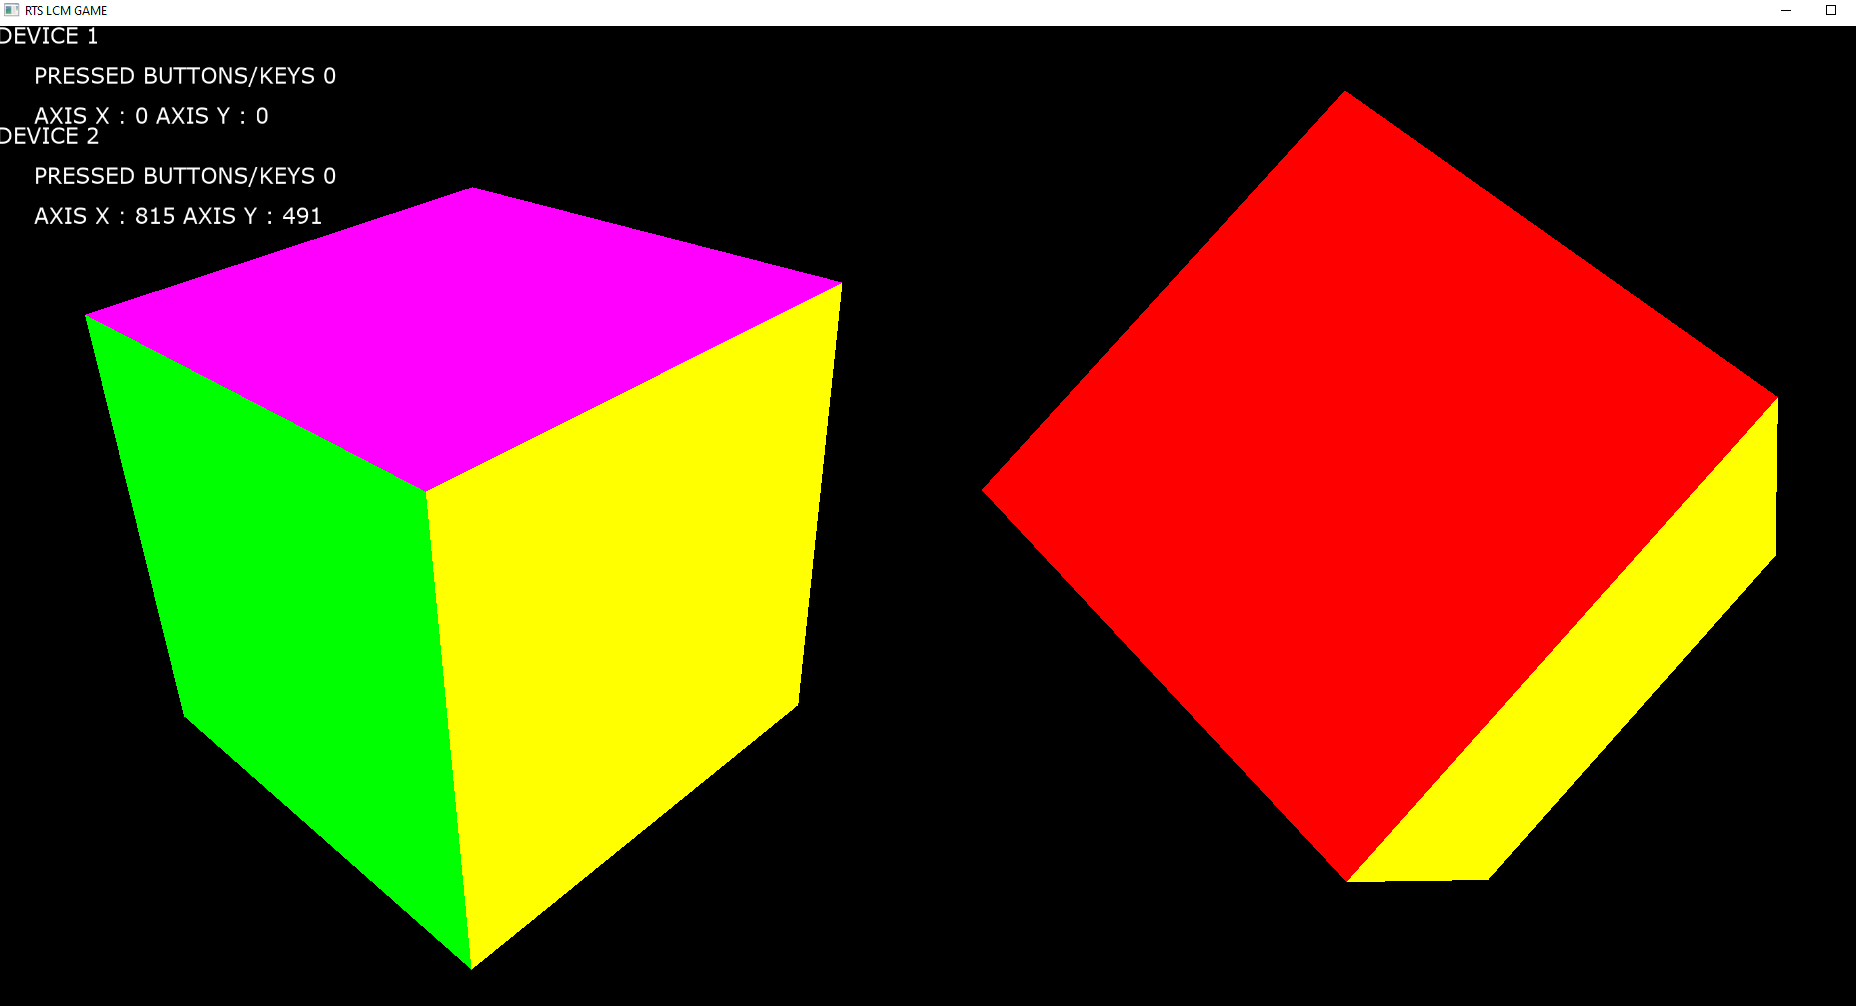
\includegraphics[width=0.7\linewidth]{screenshot004}
	\caption{a screenshot taken of the projects execution}
	\label{fig:screenshot004}
\end{figure}
This is the visible state of the project when 2 input devices are connected. both input devices have their own perspective of the cube and can control their perspective simultaneously. the debug overlay also shows the current state of each input device such as the number of pressed buttons.
\subsection {Term 2}

This is the running state of the project in Term 2. As can be seen the world map is represented as a globe
\section {Locking interaction and visibility between viewports}
\subsection {Preventing controlling other viewports UI elements}
Given the local cooperative nature of this project, it was necessary to implement safeguards preventing players from inadvertently or deliberately taking control of another player's viewport. \newline
For game controllers, this is a relatively straightforward problem to solve. Since controllers do not produce an OS-level cursor, an artificial cursor can be created programmatically and its coordinates clamped to the boundaries of the assigned viewport, effectively restricting each controller to its designated region of the screen. \newline
The mouse cursor presents a more complex challenge. Unlike a controller's artificial cursor, the OS cursor cannot be locked to a portion of the screen without introducing significant inconvenience to the user, for instance, a player may need to interact with system-level elements outside the application. As a result, free cursor movement was permitted for this project. \newline


\begin{lstlisting}[
	language=C++,
	caption={accessing a viewports owned overlay elements and excluding unowned when checking if they where pressed (\texttt{Product.sln}, 
		\texttt{OverlayController.cpp})},
	label=lst:overlay pressed checking
	]
  Ogre::Overlay* SpecificOverlay = OverlayMngr->getByName(OverlayName);

Ogre::Overlay::OverlayContainerList ContainedElements =
SpecificOverlay->get2DElements();

for (Ogre::OverlayElement* Element : ContainedElements) {
	OverlayInfo* Info = nullptr;
	try {
		Info = OverlayInfos.at(Element->getName());
	} catch (std::exception e) {
		OverlayErrorReporter.EnqueueError(
		ErrorDetail::CreateError(ErrorCode::OVERLAY_MISSING_INFO));
		return;
	}
	
	
	if (Element->findElementAt(Cntxt.MouseX, Cntxt.MouseY) && !Cmd.Released) {
		Info->Pressed = true;
		OverlayPressed(Element, Info);
	} else {
		Info->Pressed = false;
		if (Info->Hovered) {
			OverlayHovered(Element, Info);
		}
	}
}
\end{lstlisting}

As shown above, when a mouse click or trigger input is received, only the overlay elements belonging to the active viewport's assigned overlay are iterated over. This is made possible by each viewport maintaining its own dedicated overlay within Ogre3D, which can be retrieved by name to produce a list of exclusively owned overlay elements. This design offers two key benefits: it eliminates redundant checks across unrelated overlay elements, and it inherently prevents any input device from interacting with elements outside of its assigned viewport, naturally enforcing the input boundaries discussed previously. \newline

\subsection{Showing enemy units as a different colour}
Within the real time strategy genre, it's neccessary for other players to be distinguishable from one another. Most RTS games achieve this through a unique colour for each player with borders and a name tag to indicate a country.
However, due to the simplicity of the game implementation of this project there's no need for a unique colour assigned to each player and a typical player would only be concerned with having their own units be distinguishable from other players units. Therefore the chosen colour scheme for this project is white for the player themself and red for other players.

Showing other units as different colours introduces significant technical challenge. My initial thinking to solving this problem was to iterate over each entity before they're displayed on a viewport, then change their colour dynamically to reflect friendly or enemy units. This solution is however extremely inefficient since it adds an O(n) loop for each game instance, causing the render thread to slow down significantly.

My chosen approach to this problem was glsl shader program as seen below.


\begin{lstlisting}[
	language=GLSL,
	caption={glsl shader that changes a mesh's material dynamically based on the mesh's owned player id and the viewing player id (\texttt{Resources/world/mat}, \texttt{unit fp.glsl})},
	label=lst:ownership_shader
	]
	#version 330 core
	uniform float viewingPlayerID;
	uniform float ownerID;
	void main()
	{
		if (abs(ownerID - viewingPlayerID) < 0.5)
		{
			gl_FragColor = vec4(1.0, 1.0, 1.0, 1.0);
		}
		else
		{
			gl_FragColor = vec4(0.2, 0.04, 0.04, 1.0);
		}
	}
\end{lstlisting}

Rather than iterating over entities on the CPU each tick to update material states, this implementation delegates the colour logic directly to the graphics pipeline using a GLSL fragment shader. GLSL (OpenGL Shading Language) is a C-like high-level shading language that runs natively on the GPU, allowing logic to execute in parallel across thousands of cores without involving the render thread [14]. In Ogre3D, material scripts can reference GLSL programs directly, meaning this approach is not only supported natively by this project's dependencies, but also complements its concurrency-focused architecture.

This approach is considerably more suitable than iterating over entities in preViewportUpdate. The loop-based alternative requires setMaterial() to be called per entity, per tick, on the render thread — each call capable of triggering shader program rebinding, texture unit rebinding, and GPU state flushing [15]. This places the full cost of the ownership condition on the CPU, stalling the generation of the next frame until each entity is evaluated. The GLSL approach removes this responsibility from the render thread entirely, with the ownership condition resolved solely by the GPU.

A further benefit of this approach is scalability. The loop-based approach degrades linearly as entity count increases, since each additional entity causes another setMaterial() call per tick. With the fragment shader, the GPU resolves the ownerID and viewingPlayerID comparison across all relevant fragments simultaneously during rasterisation [14], meaning the CPU cost remains effectively constant regardless of how many entities are present.




\section{Project CFD}
\begin{figure}[H]
	\centering
	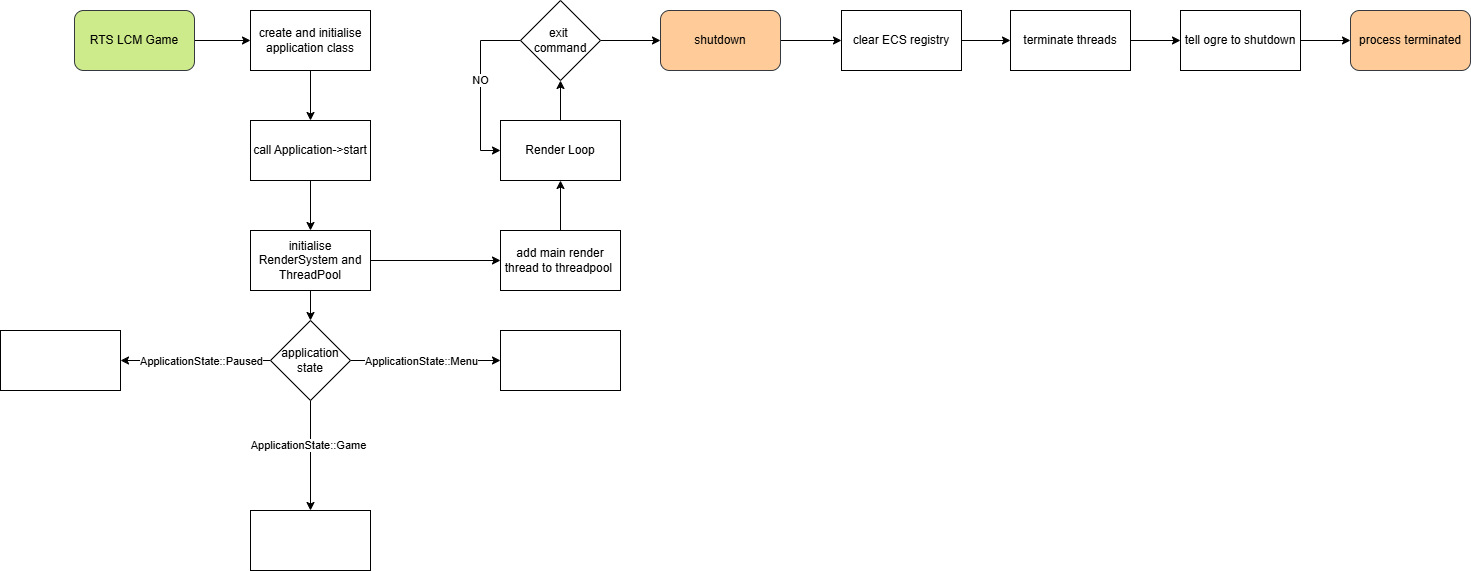
\includegraphics[width=0.7\linewidth]{../CFD}
	\caption{the control flow diagram of the projects execution. zooming in is required to read text clearly.}
	\label{fig:cfd}
\end{figure}
\chapter{performance comparisons}
\section{multi-threaded vs single-threaded}
Since the primary focus of the project is to produce a multi-threaded game I have decided to outline the relative benefit that has been achieved through using concurrency.
Below is a screenshot of the frames per second recorded in the program for the multi threaded implementation.
Below is a screenshot from a converted implementation where everything runs in the main thread.

There are, however, some important limitations of this comparison to consider. 
The most fundamental is that this project was designed specifically around 
multi-threading, meaning the event architecture approach is entirely 
inappropriate for a single threaded environment and inherently favours 
multi-threaded execution. Event architecture with event queues introduces 
additional overhead in a single threaded conversion, since events are still 
enqueued and dispatched despite these steps being entirely unnecessary in a 
single threaded context where no race conditions can occur. This overhead 
penalises the single threaded version in a way that is structurally unfair, as 
it measures the cost of a concurrency solution in an environment where 
concurrency is not present.

A further limitation is that a large number of objects within this project are 
allocated to the heap. This is a deliberate design decision in the multi-threaded 
implementation, as heap allocation allows for cleaner ownership and lifetime 
management across threads. In a single threaded environment, however, this 
becomes unnecessary. Classes that currently operate on instance threads, such as 
\texttt{InputListener}, could instead be processed within the same call stack, 
allowing stack allocation or direct in-place processing, both of which carry 
considerably less overhead than repeated heap allocation.

A third limitation concerns thread overhead itself. NVIDIA's technical 
documentation notes that many CPU-bound applications degrade in performance as 
thread count increases, citing hardware resource contention, increased pressure 
on the memory subsystem, and higher rates of OS context switching as contributing 
factors [7]. The single threaded version of this project 
introduces exactly these kinds of artefacts via the event architecture without 
receiving any of the parallelism benefits that justify them, further skewing the 
comparison against the single threaded implementation.

Taken together, these limitations mean that a fair and meaningful comparison 
between a multi-threaded and single threaded version of this project would 
require a ground-up redesign of the single threaded implementation to better 
suit that execution model. This would involve replacing the event queue 
architecture with direct function calls, reducing unnecessary heap allocation, 
and restructuring subsystems such as \texttt{InputListener} to operate without 
thread boundaries. Such a redesign would be too time consuming given the time 
constraints of this project and falls outside its intended scope.


\chapter {deployment}

\section {deployment prerequisites}
 
\textbf{at a bare minimum you should possess:} \newline
- an x64 based cpu 
- an operating system compatible with OpenGL or DirectX
- at least one games controller to test the split screen functionality
- a modern dedicated GPU, preferably one with more than 4gb of video memory.
 
\textbf{additionally, before deploying this project please ensure you have installed and configured the following:} \newline
-  Visual studio Community edition 2022
-  the vcpkg component of visual studio 


details on how to install and configure the above can be found in the deployment video provided in the git repository.
\section{deployment instructions}

* open product.sln (if a retarget prompt appears then refer to deployment perquisites) \newline
* this project uses cpplint in pre build events, run "pip install cpplint" (important that this is done in the vs python command prompt and not a regular command prompt) \newline
* you'll be presented with 3 different projects in visual studio, "product" is a static lib and "tests" + "application" is an exe \newline
* before compiling, configure "multiple startup projects" and make sure that the static lib isn't run but the other 2 are \newline
* clean then rebuild all using visual studio, vcpkg will download and install dependencies (usually takes ~2-~3 hours) \newline
* Please note that if the first run fails it means that vcpkg automatic linking failed. as a fallback, post build events will copy all required DLLs to the output dir meaning the second run wont fail. \newline
* Please note that this project requires OpenGL to be installed, the glsl shader will not function when this project is used with DirectX
* *VERY IMPORTANT* if you are running my project from inside visual studio you must change the debugging directory (working directory in the debugging section) for each individual project (application, product, tests)  to \$(OutDir) (must be uniform between projects), prebuild events will copy the right ogre config to the outdir so please keep in mind if you decide to build my project to a different directory (outside of visual studio) then you need to recreate this behaviour.\newline

\section{changes to the deployment process in term 2}



\chapter{Software engineering methodologies}
\section{testing environment}
This project uses the Doctest C++ library for unit testing with Cpplint to check for google c++ style compliance.To test for memory leaks and concurrent performance within my project im using the native visual studio debugger with Open Hardware Monitor to check core utilization.

This project is tested on 2 different computers

\textbf{Primary development computer } \newline
\textbf{Operating System:} Windows 11 Home edition \newline
\textbf{CPU:} Ryzen 9 9950X3D \newline
\textbf{GPU:} Nvidia RTX 5090 \newline
\textbf{RAM:} 64GB DDR4 \newline
disk running and storing project: Nvme SSD \newline

\textbf{secondary development computer} \newline
\textbf{Operating System:} Linux Mint with Wine installed \newline
\textbf{CPU:} Ryzen 7 3700x \newline
\textbf{GPU:} AMD Radeon 7700XT \newline
\textbf{RAM:} 16GB DDR4 \newline
disk running and storing project: standard sata SSD \newline

\textbf{both running at factory clock rates} \newline

\section{Use of TDD}
This project was developed using a structured and methodical approach to modern software engineering practices.using industry standard system design from both a Game development and a concurrency standpoint, My Deployment process is also streamlined for rapid deployment with unit testing done to ensure correctness. Unit tests are automatically run alongside this project when run inside visual studio meaning i can easily identify if a new feature has affected previous functionality, alongside this cpplint is run as a prebuild event to check for google c++ standard compliance.
\section{system architecture}
This project uses Event architecture and Entity Component System, an industry standard pattern for game development. Event architecture has allowed this project to reduce class coupling since classes communicate via events instead of direct access. Event queues also manage race conditions since events are processed in serial rather than having two conflicting events running in parallel. 

Another architectural standard this project follows is Thread pooling, this is an industry standard approach to concurrency as it allows consistent hardware utilization across cpu cores. 

throughout the development of this project, a control flow diagram was updated regularly to show the codes execution.

\section{Version control}
This project uses Git as a version control solution, with the Git repository being hosted on the department git lab. Progress was frequently committed throughout the development process and the main branch was kept in a working state throughout to keep a restore point available. major changes to this project where created on seperate branches with branch objectives set before hand, before merging into main the feature branch is thoroughly tested and checked against branch objectives.
\newpage
\chapter{Acronomys}
\textbf{ECS - }Entity Component System \newline
\textbf{REA - }Resource Entity Action \newline
\textbf{RTS - }Real Time Strategy \newline
\textbf{SDL2 - }Software Direct Media Layer \newline
\textbf{LCM - }Local Multi Player \newline
\textbf{CPU - }Central Processing Unit \newline
\textbf{GPU - }Graphical Processing Unit \newline
\textbf{RAM - }Random Access Memory \newline
\textbf{TDD - }Test Driven Development \newline
\textbf{GUI - }Graphical user interface \newline
\textbf{GUI - }Graphical user interface \newline
\newpage{GLSL - }OpenGL shading language\newline
\newpage{HLSL - }High level shading language\newline
\newpage{MSL - }Metal shading language\newline
\newpage{WGSL - }WebGPU shading language\newline
\chapter{Glossary}
\textbf{Ogre3d - }a lightweight rendering engine in the form of a c++ library \newline
\textbf{Ogre Overlay -} a component included inside the Ogre3d ecosystem, focused on overlaying 2d objects over a 3d viewport \newline
\textbf{Dear Imgui - }a c++ rendering library focused on creating debug overlays \newline
\textbf{Software Direct Media Layer -} a commonly used cross platform input handling library for c++ \newline
\textbf{Resource Entity Action - }a design pattern for real time strategy games that 
models entity interactions into transformation matrices that define resource exchanges between entities for fast evaluation \newline
\textbf{Entity Component System - }a software architecture pattern that separates
game objects into entities (identifiers) and components (pure data containers).
ECS is used where composition is prioritized over inheritance \newline
\textbf{entt - }an Entity Component System library for C++ that uses sparse set to
store entities \newline
\textbf{nlohmann json-} a popular JSON library in c++ \newline
\textbf{stellaris} a real time strategy game from Paradox interactive, known to have performance issues \newline
\textbf{Fragment shader} A programmable stage of the rendering pipelines, running for each pixel on the screen\newline


\chapter{bibliography}
[1] Colson, D. (2020) How to make a simple entity-component-system in C++. Available at: \url{https://www.david-colson.com/2020/02/09/making-a-simple-ecs.html} (Accessed: 10th November 2025). \newline

[2] Abbadi, M., Di Giacomo, F., Orsini, R., Plaat, A., Spronck, P. and Maggiore, G. (no date) Resource Entity Action: A Generalized Design Pattern for RTS games. Università Ca' Foscari DAIS - Computer Science, Venice, Italy; Tilburg University, Netherlands; NHTV University of Applied Sciences, Breda, Netherlands. Available at: \url{https://liacs.leidenuniv.nl/~plaata1/papers/abbadi-resources_entities_actions_a_generalized_design_pattern-118.pdf} (Accessed: 10th December 2025). \newline

[3] Epic Games (2025) Nanite Virtualized Geometry in Unreal Engine. Unreal Engine 5.7 Documentation. Available at: \url{https://dev.epicgames.com/documentation/en-us/unreal-engine/nanite-virtualized-geometry-in-unreal-engine} (Accessed: 5th December 2025). \newline

[4] Microsoft (2025) GameInput introduction - Overview of GameInput. Microsoft Game Development Kit. Available at: \url{https://learn.microsoft.com/en-us/gaming/gdk/docs/features/common/input/overviews/input-overview} (Accessed: 25th September 2025). \newline

[5] Cox, L., Williams, B., Vickers, J., Ward, D. and Headleand, C. (2025) 'Run-time Performance Comparison of Sparse-set and Archetype Entity-Component Systems', in Sheng, Y. and Slingsby, A. (eds.) Computer Graphics and Visual Computing (CGVC). The Eurographics Association. Available at: \url{https://diglib.eg.org/server/api/core/bitstreams/766b72a4-70ae-4e8e-935b-949d589ed962/content} (Accessed 10th December 2025). \newline

[6] Compton, B.V. (2022) An Investigation of Data Storage in Entity-Component Systems. Master of Science thesis. Air Force Institute of Technology. Available at: \url{https://scholar.afit.edu/etd/5353/} (Accessed: 5th December 2025). \newline

[7] NVIDIA Corporation (2024) Limiting CPU threads for better game performance. 
NVIDIA Technical Blog. Available at: 
\url{https://developer.nvidia.com/blog/limiting-cpu-threads-for-better-game-performance/} 
(Accessed: 17th March 2026). \newline

[8] GeeksforGeeks (2025) Map vs unordered\_map in C++. Available at: \url{https://www.geeksforgeeks.org/cpp/map-vs-unordered_map-c/} (Accessed: 4th November 2025). \newline
[9] GeeksforGeeks (2025) set vs unordered\_set in C++ STL. Available at: \url{https://www.geeksforgeeks.org/cpp/set-vs-unordered_set-c-stl/} (Accessed: 4th November 2025). \newline
[10] GeeksforGeeks (2025) Advantages of vector over array in C++. Available at: \url{https://www.geeksforgeeks.org/cpp/advantages-of-vector-over-array-in-c/} (Accessed: 4th November 2025). \newline
[11] SDL Community (2004) Case sensitive key down? Simple DirectMedia Layer Development Forum. Available at: \url{https://discourse.libsdl.org/t/case-sensitive-key-down/10807} (Accessed: 5th November 2025). \newline
[12] Stack Overflow (2023) fmt compile-time format string check without generating ASM code for the check. Stack Overflow. Available at: \url{https://stackoverflow.com/questions/76329898/fmt-compile-time-format-string-check-without-generating-asm-code-for-the-check} (Accessed: 7th November 2025). \newline
[13] OGRECave (2025) Ogre 3D Engine --- Simple samples. GitHub. Available at: \url{https://github.com/OGRECave/ogre/tree/master/Samples/Simple/include} (Accessed: 8th November 2025). \newline
[14] Wikipedia (2026) OpenGL Shading Language. Wikipedia. Available at: \detokenize{https://en.wikipedia.org/wiki/OpenGL_Shading_Language} (Accessed: 5th April 2026).
[15] Generalist Programmer (2025) Shader Programming Complete Graphics Guide 2025: Master Real-Time Rendering. Available at: https://generalistprogrammer.com/tutorials/shader-programming-complete-graphics-guide-2025 (Accessed: 5th April 2026).
[16] Galvan, A. (2024) A Review of Shader Languages. Alain.xyz. Available at: https://alain.xyz/blog/a-review-of-shader-languages (Accessed: 8th April 2026).
[17] Wikipedia (2025) Shading language. Wikipedia. Available at:\detokenize{https://en.wikipedia.org/wiki/Shading_language} (Accessed: 8th April 2026).
[18] Khronos Group (2015) Fixed Function Pipeline. OpenGL Wiki. Available at: \detokenize{https://wikis.khronos.org/opengl/Fixed_Function_Pipeline} (Accessed: 8th April 2026).
[19] Quilez, I. (2018) \textit{Raymarching Distance Fields}. iquilezles.org. Available at: https://iquilezles.org/articles/raymarchingdf/ (Accessed: 8th April 2026).
[20] Quilez, I. (2010) \textit{Soft Shadows in Raymarched Signed Distance Fields}. iquilezles.org. Available at: https://iquilezles.org/articles/rmshadows/ (Accessed: 8th April 2026).
\newpage
\chapter{appendices}
\section{project diary}
11/10/25 - researched convenient way to implement TDD
11/10/25 - configured and succesfully setup project
12/10/25 - configured cpplint to check c++ google standard
12/10/25 - designed general structure of ECS Registry and Event bus
12/10/25 - created initial test templates
12/10/25 - created EventBus and EventQueue tests
13/10/25 - researched ogre render system patterns
13/10/25 - initial ViewPortController and RenderSystem classes and tests
14/10/25 - investigated the best way of harvesting input simultaneously from multiple controllers (arrived at SDL2, integrated into ogre by default)
15/10/25 - created initial event templates and InputListener class
15/10/25 - shifted focus to ECS storage, researched how entt registry should be managed and who should own it. decided on a WorldManager singleton
16/10/25 to 19/10/25 - modeling runtime scripts and researching other ogre3d projects
20/10/25 - race condition tests, initial implementation of runtime scripts using app states
21/10/25 - write base renderSystem class, designed error and logging system 
22/10/25 - wrote EventBus and EventQueue class as prequisite to error and logging system 
22/10/25 - realised EventQueue class erases type information, redesigned and placed queue items in a wrapper class
24/10/25 - wrote passing tests for eventQueue
25/10/25 - when doing ogre runtime tests i realised that the vcpkg version of ogre is incorrect, porting fully to a manual build
26/10/25 - identified that the issue was due to string corruption of the package name, ported back to vcpkg and fixed by linking debug libraries when neccessary
27/10/25 - wrote passing viewport tests (apart from an unidentified issue regarding viewport z-orders)
28/10/25 - passing tests across the board (bar 2 viewport tests), created a responsive ogre render window
29/10/25 - integrated and initialised SDL2 and Dear Imgui
30/10/25 - partial implementation of error reporting (without handling yet)
30/10/25 - looked at sample programs in the ogre and sdl doc, realised input listener cant be on a per instance basis, redesigned such that a singular input handler dispatches to each instance
31
4/11/25 - which data structure and key is appropriate for having an input device bound to an sdl id? (same issue for input device and queue)
4/11/25 - read \detokenize{https://www.geeksforgeeks.org/cpp/map-vs-unordered_map-c/}
4/11/25 - \detokenize{read https://www.geeksforgeeks.org/cpp/set-vs-unordered_set-c-stl/}
4/11/25 - read https://www.geeksforgeeks.org/cpp/advantages-of-vector-over-array-in-c/
4/11/25 - settled on unordered set instead of vectors, mainly for O(1) lookups but also since its a set and it only needs to store unique data
5/11/25 - how can i replicate case sensitivy for sdl when sdl2 doesnt generate capital letter events? 
5/11/25 - read https://discourse.libsdl.org/t/case-sensitive-key-down/10807
5/11/25 - realized sdl2 has global "mod" events, used them to check for shift and capslock state to replicate case sensitivity
6/11/25 - test port to secondary pc
6/11/25 - realized that plugins.cfg used by ogre reads exclusively from the build output dir which isnt replicated on gitlab
6/11/25 - added a prebuild event to copy from product/ to (Outdir)
7/11/25 - how can i add specific error information for my error handling?
7/11/25 - used previously familiar format library
7/11/25 - encountered issue where format would read string values at compile time as const
7/11/25 - realized limitation of format library with a static lib and researched alternatives
7/11/25 - read https://stackoverflow.com/questions/76329898/fmt-compile-time-format-string-check-without-generating-asm-code-for-the-check
7/11/25 - implemented fmt library instead as dependancy then used fmt in CreateError calls to force runtime string building
8/11/25 - researched Imgui implementation and consulted ogre doc with imgui example at https://github.com/OGRECave/ogre/tree/master/Samples/Simple/include
8/11/25 - realized this example didnt apply to me due to their use of ApplicationBase (used to make cookie cutter ogre3d apps not relevant to me )
8/11/25 - attempted custom implementation of imgui in my project, repeated failure
8/11/25 - consulted countless forum posts on the ogre forum, many outdated and irrelevant to the issue
8/11/25 - realized imguis IO string fields "BackEndRenderer" was corrupt/inaccesible
9/11/25 - realized that im building imgui and ogre as dynamic library with no way of accessing a shared IO
9/11/25 - edited project properties to build as static lib (for unified memory)
9/11/25 - major edits to project setup for compatibility with static lib versions of ogre and sdl2 etc
10/11/25 - using ogre in static lib mode proved to be a major pain, reverting back to last stable build
10/11/25 - after revert, used native ogre overlay support to add OverlayController (class owned by RenderSystem and is responsible soley for overlays)
11/11/25 - stopped checking controller GUID, realised it was manufacturer id and anyone using generic controllers (like me) would have their controllers lumped onto the same id
11/11/25 - added a debug overlay that shows activity of all input devices
11/11/25 - when refining before final merge, i noticed that SDL2 actually has a limitation with generic controllers, that being it has literally no idea which is which, this isnt a problem if they dont disconnect but finding the right controller to connect back to is now proving extremely difficult
11/11/25 - my first idea for solving this problem is to just reconnect controllers to the slot that doesnt have a valid controller connected, this would work perfectly fine however a foreseeable issue is if two controllers disconnect at the same time then they may end up in the wrong slot. this is the most practical solution for now however once the project is at a later stage my definitive solution is to have a prompt pop up for each disconnected user saying "press any key (player)" so the user can manually put it back in the right slot
11/11/25 - implemented fix to controller reconnection, as suspected theres an issue where disconnected 2 controllers can cause the slots to switch
12/11/25 - noticed that the input sensitivity of controllers depended on the frame rate the game was running on when testing on multiple clamped frame rates
12/11/25 - implemented a dynamic delta time value that can easily be retrieved from RenderSystem and scaled input sensitivity with it
13/11/25 - 22/12/25 - time dedicated to multiple assignments for other modules
23/11/25 - asked myself what should i be doing for users with different display types or render preferences
24/11/25 - utilized nlohmann json to make a generic ConfigManager usable for any config elsewhere in my codebase
25/11/25 - implemented the new config system for video settings, including render resolution, the default render resolution is 1920x1080 since its the most common resolution
27/11/25 - researched ECS implementations for use cases similar to mine
28/11/25 - researched the ogre docs to see what information i should be storing for my ECS entities
29/11/25 - initial ECS implementation with a test cube (different coloured faces) for the demo

12-20/12/25 - final refinements to interim report (extension used)

--- out of term development 
12/12/25 - research similar split overlay implementations (having overlays unique to a viewport)
14/12/25 - implemented extended functionality to rendersystem through an owned class (PreViewPortUpdateListener)
15/12/25 - implemented unique overlay functionality by hiding other overlays at the precise moment they are about to rendered, this is done using the PreViewPortUpdate event thats dispatched automatically by ogre

27/12/25 - limit the cursor position to the size of a unique overlay, this functionality will be extended in future by preventing the cursor from moving over other viewports

--- term 2 start
19/01/26 - revisited \detokenize{https://liacs.leidenuniv.nl/~plaata1/papers/abbadi-resources_entities_actions_a_generalized_design_pattern-118.pdf} for a better understanding of resource entity action
20/01/26 - wrote failing tests for the transformation matrix class
20-25/01/26 - implementation of a rudimentary cursor implementation, noticed significant stability issues from this implementation
26/01/26 - following testing of the cursor implementation, i decided that sticking to the default OS cursor for mouse was a better option for the mouse but keeping the system in place for controllers
27/01/26 - refactored the dispatching order for events such that events are processed the same frame they are created, reducing the perceived delay from the cursor
28/01/26 - created the entity interaction class, a class thats responsibility is to process all entity interactions and route matrixable interactions accordingly.
29-31/01/26 - edge cases for matrix tests, stability improvements following detailed analysis from performance profiler.

02/02/26 - read https://stackoverflow.com/questions/26516683/reusing-thread-in-loop-c to learn about reusing threads
02/02/26 - added BS thread pool as a dependancy, implemented into the current thread pool pattern, improved fps and stability remarkability (500->2000fps) and cpu usage of the gameinstance->run method dropped from 12.8% of 1 core to 2.7%
03/02/26 - noticed another significant performance limiter, updated application->run to follow the updated threading model and increased fps from 2000fps to 6000fps (cpu time dropped from 2.7% to 1.3%)

9/02/26 - designed an initial game map implementation, attempting to replicate the world map as a single mesh
10/02/26 - after experimenting with the initial game map, i realised a cleaner approach would be to seperate the land masses as distinct meshes. this realisation came after investigating the ogre doc, specifically the ray tracing functionality. since ogre ray tracing handles mesh collision checks automatically, having the land masses be seperate meshes was a clean way of identifying land the units could spawn on (land masses) and ones they couldnt (the sea)
11/02/26 - redesigned the world map after taking this into account, with countries also pertruding from the sea for an easier time with ogre raytracing.
12/02/26 - updated world manager to load the new globe, each country is added to the same scenenode to make moving the globe easier if need be. the implemented world map does have a couple rendering errors, that being that some countries are visible through the globes surface (when the camera is facing the other side of the globe)

16/02/26 - investigated how input translator currently propogates input events
17/02/26 - realized that input translator up until this point has mainly been focused on only communicating with the same instance thread it runs in (input events arent sent elsewhere but instead the instance thread reads the states manually)
18/02/26 - designed a new struct for input events sent to the render thread to be identifiable back to the instance thread it was sent from (ActionContext), along with other context such as on a MousePressed event it includes the screen coordinates pressed and whether the button was pressed for the first time or is being held down (instead of a MousePressed event only indicating that that device was pressed and nothing else)

27/02/26 - looked into how to fix the rendering errors present from the globe implementation. read https://forums.ogre3d.org/viewtopic.php?t=81112
28/02/26 - since ive been using blender for my 3d meshes, the z order should be managed automatically so i deduced that the materials are the issue
28/02/26 - read https://forums.ogre3d.org/viewtopic.php?t=57151 to identify the issue
28/02/26 - added a depth \detokenize{pre_pass} level to the material scripts for the country material, this fixed the issue

6/03/26 - setup for raytracing functionality, initialised an Ogre:rayscenequery on startup
7/03/26 - using the new functionality in input translator, Player general control now starts a raytrace when the mouse is pressed. the result isnt used yet but has been verified to be correct for future implementation

9/03/26 - revisited older overlay code to try and figure out a clean method to add pressable buttons
10/03/26 - decided on using a callback system for button functionality, buttons would register an event to be queued back to an event queue pointer once the button was clicked allowing OverlayController to handle all of the mouse hovering and mouse pressed checks.
11/03/26 - implemented the new functionality into overlaycontroller and added a new button class to make adding a functional button easier (GenericButton.cpp)

14/03/26 - implemented a basic state machine in preparation for a main menu
15/03/26 - using the new button class (Generic button) i created a main menu button that issues ChangeState event when pressed
15/03/26 - added functionality to rendersystem to hide or show a mesh when needed, allowing me to hide the globe by default then show the globe when the play button is pressed

20/03/26 - using previously unintegrated raytracing functionality, players can now select a unit or city
20/03/26 - added functionality to highlight the selected unit or city by changing its colour to red
21/03/26 - extended selection functionality by only allowing one city or unit to be selected, and pressing on a valid land mass will store the coordinates for future movement

22/03/26 - added movement functionality to units, using the stored coordinates then the interaction wheel to move them

25/03/26 - enemy units now appear as a different colour, this was done using a glsl fragment shader that does the ownership check on the gpu. units and cities now use a new material. \detokenize{unit_fp} that includes this check and once their initialised they have their ownership stored within it

26/03/26 - added a new entity component, ProducesUnitsComponent. in the entitiy loop, this component adds to the available units passively




\end{document}
